Monocular depth estimation is a well-explored, yet active area of research (see Sec.~\ref{sec:related}). Any network trained for the MDE task takes as input an RGB image and estimates the depth map of the scene. Our approach augments existing MDE networks but is agnostic to the specific type of depth estimator. Indeed we show in Section~\ref{sec:evaluation} that our histogram matching technique equally improves a variety of different pre-trained estimators. In the remainder of this section, we therefore focus on modeling the image formation of a diffused single-photon avalanche diode (SPAD) and develop an approach to correcting an estimated depth map to match the global scene information captured by the SPAD.

%In this section, we describe the measurement model for a single-pixel time-of-flight lidar sensor under diffuse, pulsed laser illumination. 

%%%%%%%%%%%%%%%%%%%%%%%%%%%%%%%%%%%%%%%%%%%%%%%%%%%%%%%%%%%%%%%%%%%%%%%%%%%%%%%%%%%%%%%%%%%%%%%%%%%%%%%%%%%%%%%%%%%%
\subsection{Image Formation Model of a Diffused SPAD}

Consider a diffused laser that emits a pulse at time $t = 0$ with time-varying intensity $g(t)$ illuminating some 3D scene. We parameterize the geometry of the scene as a height map $z(x, y)$, where each of the 3D points has also some unknown reflectivity $\alpha$ at the wavelength of the laser. Ignoring interreflections of the emitted light within the scene, a single-pixel diffused SPAD then integrates all the light scattered back from the scene towards the detector as
%
\begin{equation}
	s \left( t \right)= \int_{\Omega_x} \int_{\Omega_y} \alpha \left( x,y \right) g \left( t - \frac{2z(x,y)}{c} \right) dx dy ,
	\label{eq:pulse_integral} 
\end{equation}  
%
where $c$ is the speed of light and $\Omega_{x,y}$ is the angular range of the diffuser. In this formulation, $\alpha$ also absorbs the square distance falloff of light and we assume that the diffuser spreads light uniformly over all angles. Each time such a light pulse is emitted into the scene and scattered back to the detector, the single-pixel SPAD time-stamps up to one of the returning photons with some probability. This is not necessarily the first returning photon. The process is repeated millions of times per second with the specific number of emitted pulsed being controlled by the repetition rate of the laser, which is typically adjusted to match the deadtime of the SPAD~\cite{Heide:2018}. Each detected photon arrival event is discretized into a histogram $h$ of the form
%
\begin{equation}
  h[n] \sim \mathcal{P} \left( \eta \int_{n\Delta t}^{(n+1)\Delta t} \left(f * s \right) \left( t \right)  dt + b \right),	
	\label{eq:spad_measurements}
\end{equation}
%
where $(n\Delta t, (n+1) \Delta t)$ models the $n^{th}$ time interval of the temporal histogram, $\eta$ is the photon detection probability of the SPAD, $f$ is a function that models the temporal uncertainty in the detector, and $b$ represents ambient background light and falsely detected photons known as dark count. As derived in previous work, the combination of signal, background, and noise can be modeled as an inhomogeneous Poisson process $\mathcal{P}$~\cite{Kirmani:2014,Shin2015}.

\paragraph{SPAD Denoising}
To remove the ambient and dark count photons from the histogram, we apply a
preprocessing step. First, we compute an estimate of the combined ambient
and dark count rate $\hat b$ by averaging $N$ of the first bins together. We then
note that that shining a laser through a 2D diffuser and
measuring a single pixel is very physically similar to recording a single 
non-line-of-sight measurement. We
compute the first difference of the histogram and find the first and last edges 
$i_{first}$ and $i_{last}$ where $\abs{h_i - h_{i+1}}$ is
significantly larger than what would be expected given the rate $b$. From
\cite{Xin2019}, these edges
correspond to the discontinuties in the depth map 
at the closest and furthest image depths, and therefore all of the signal
photons must be in the bins between these two edges. We refine these estimates by
computing $i'_{first} = \max_{i}\mset{i}{h_i > \hat b, i < i_{first}}$ and
$i'_{last} = \min_{i} \mset{i}{h_i > \hat b, i > i_{last}}$
Finally, we reject all photons outside of the valid range by clamping those bins
to 0, and we subtract our ambient estimate from the photons within the valid
range, giving a denoised histogram
\[(h_{denoised})_i = \begin{cases}
    0 & i < i'_{first} \\
    max(h_i - \hat b, 0) & i'_{first} \leq i \leq i'_{last} \\
    0 & i > i'_{last} \\
  \end{cases}.\]
% \begin{itemize}
%   \item Talk about histogram matching in the ideal case, jump straight to intensity 
%   \item Talk about histogram matching in our case, and how it approaches the
%     ideal case. Discuss the following corrections 
%     \begin{itemize}
%       \item Ambient/DC - Use \cite{Xin2019} to justify looking for large edges,
%         then the ambient estimate to get rid of the noise floor.
%       \item Falloff
%     \end{itemize}
%   \item Talk about how the histogram matching works with intensity
%     considerations applied, briefly.
%   \item We don't address jitter or poisson noise.
% \end{itemize}
% \begin{equation}
%   h[n] \sim \mathcal{P}\paren*{\sum_{x,y}\alpha_{x,y}\eta \lambda_{x,y}[n] + b} \label{global_hints}
% \end{equation}
% Given a SPAD with histogram $h$ according to the above equation, we first
% process the SPAD to remove the effects of some of the terms. First, we 


%Neglecting albedo and falloff effects, an ideal detector counting photon events
%from a location $(x,y)$ in the time interval $(n\Delta t, (n+1) \Delta t)$ would record
%
%\begin{equation}
  %\lambda_{x,y}[n] = \int_{n\Delta t}^{(n+1) \Delta t} (f * g)\paren*{t - 2z(x,y)/c} dt \label{single_loc_spad} 
%\end{equation}  
%
%where $c$ is the speed of light, and $f$ is a function that models the temporal uncertainty in the
%detector. Single-photon avalanche diodes (SPADs) are highly sensitive
%photodetectors which are able to record single photon events with high temporal
%precision \cite{Stuff}. Since the event corresponding to the detection of a
%photon can be described with a Bernoulli random variable,
%the total number of accumulated photons in this time interval follows a Poisson
%distribution according to
%
%\begin{equation}
  %h[n] \sim \mathcal{P}\paren*{\sum_{x,y}\alpha_{x,y}\eta \lambda_{x,y}[n] + b} \label{global_hints}
%\end{equation}
%
%where $\alpha_{x,y} = r_{x,y}/z(x,y)^2$ captures the attenuation of the
%photon counts due to the reflectance $r(x,y)$ of the scene and due to the
%inverse square falloff $1/z(x,y)^2$.
%In addition, $\eta$ is the detection probability of a photon
%triggering a SPAD event, and $b = \eta a + d$ is the average number of background detections resulting
%from ambient photons $a$
%and erroneous ``dark count'' events $d$ resulting from noise within the SPAD.
%% \newpage
%% \begin{table*}[htbp]
%%   \begin{center}
  %%   \begin{tabularx}{\linewidth}{*{2}{X}}
  %%     \includegraphics[width=\textwidth/2-5pt]{sections/figures/spad_example/rgb.png} &
  %%     \includegraphics[width=\textwidth/2-5pt]{sections/figures/spad_example/rawdepth.png} \\
  %%     \includegraphics[width=\textwidth/2-5pt]{sections/figures/spad_example/depth_hist.png} &
  %%     \includegraphics[width=\textwidth/2-5pt]{sections/figures/spad_example/spad_hist.png} \\
  %%   \end{tabularx}
  %% \end{center}
  %% \caption{Sample Image. Top Left is the RGB image. Top Right is ground truth
  %%   depth. Bottom Left is Raw ground truth depth histogram. Bottom Right is
  %%   simulated SPAD measurements. Notice how closer depths are magnified and far
  %%   depths are attenuated.}
%% \end{table*}
%
%%%%%%%%%%%%%%%%%%%%%%%%%%%%%%%%%%%%%%%%%%%%%%%%%%%%%%%%%%%%%%%%%%%%%%%%%%%%%%%%%%%%%%%%%%%%%%%%%%%%%%%%%%%%%%%%%%%%
\subsection{Monocular depth estimation with global depth hints}
Given a single RGB image $I(x,y)$ and a vector of photon arrivals $h[n]$
described by equation \ref{global_hints}, we seek to
reconstruct the ground truth depth map $z(x,y)$.
Our method has two parts. First, we \textbf{initialize} our estimate of the depth map from the single RGB
image via a monocular depth estimator described below. Second, we \textbf{refine} this depth map using
the captured measurements $h[n]$ via exact histogram matching. 

\paragraph{Initialization}
The first step in our method is to produce an initial estimate of ground truth
depth. Convolutional Neural Networks have been shown to produce accurate, if poorly-scaled, estimates of depth
from only a single image. We therefore choose to initialize our depth map
estimate $\hat z^{(0)}(x,y)$ using
a CNN. However, any depth estimator reliant on only a single
view may be used for this step. Furthermore, in the larger context of our
algorithm, it is more important that the network predict the correct ordinal
relationships between pixels - that is, to predict the correct relative ordering
of pixels $a$ and $b$, rather than to get all pixels exactly correct.

\paragraph{Exact Histogram Matching}
\begin{figure*}
  \centering
  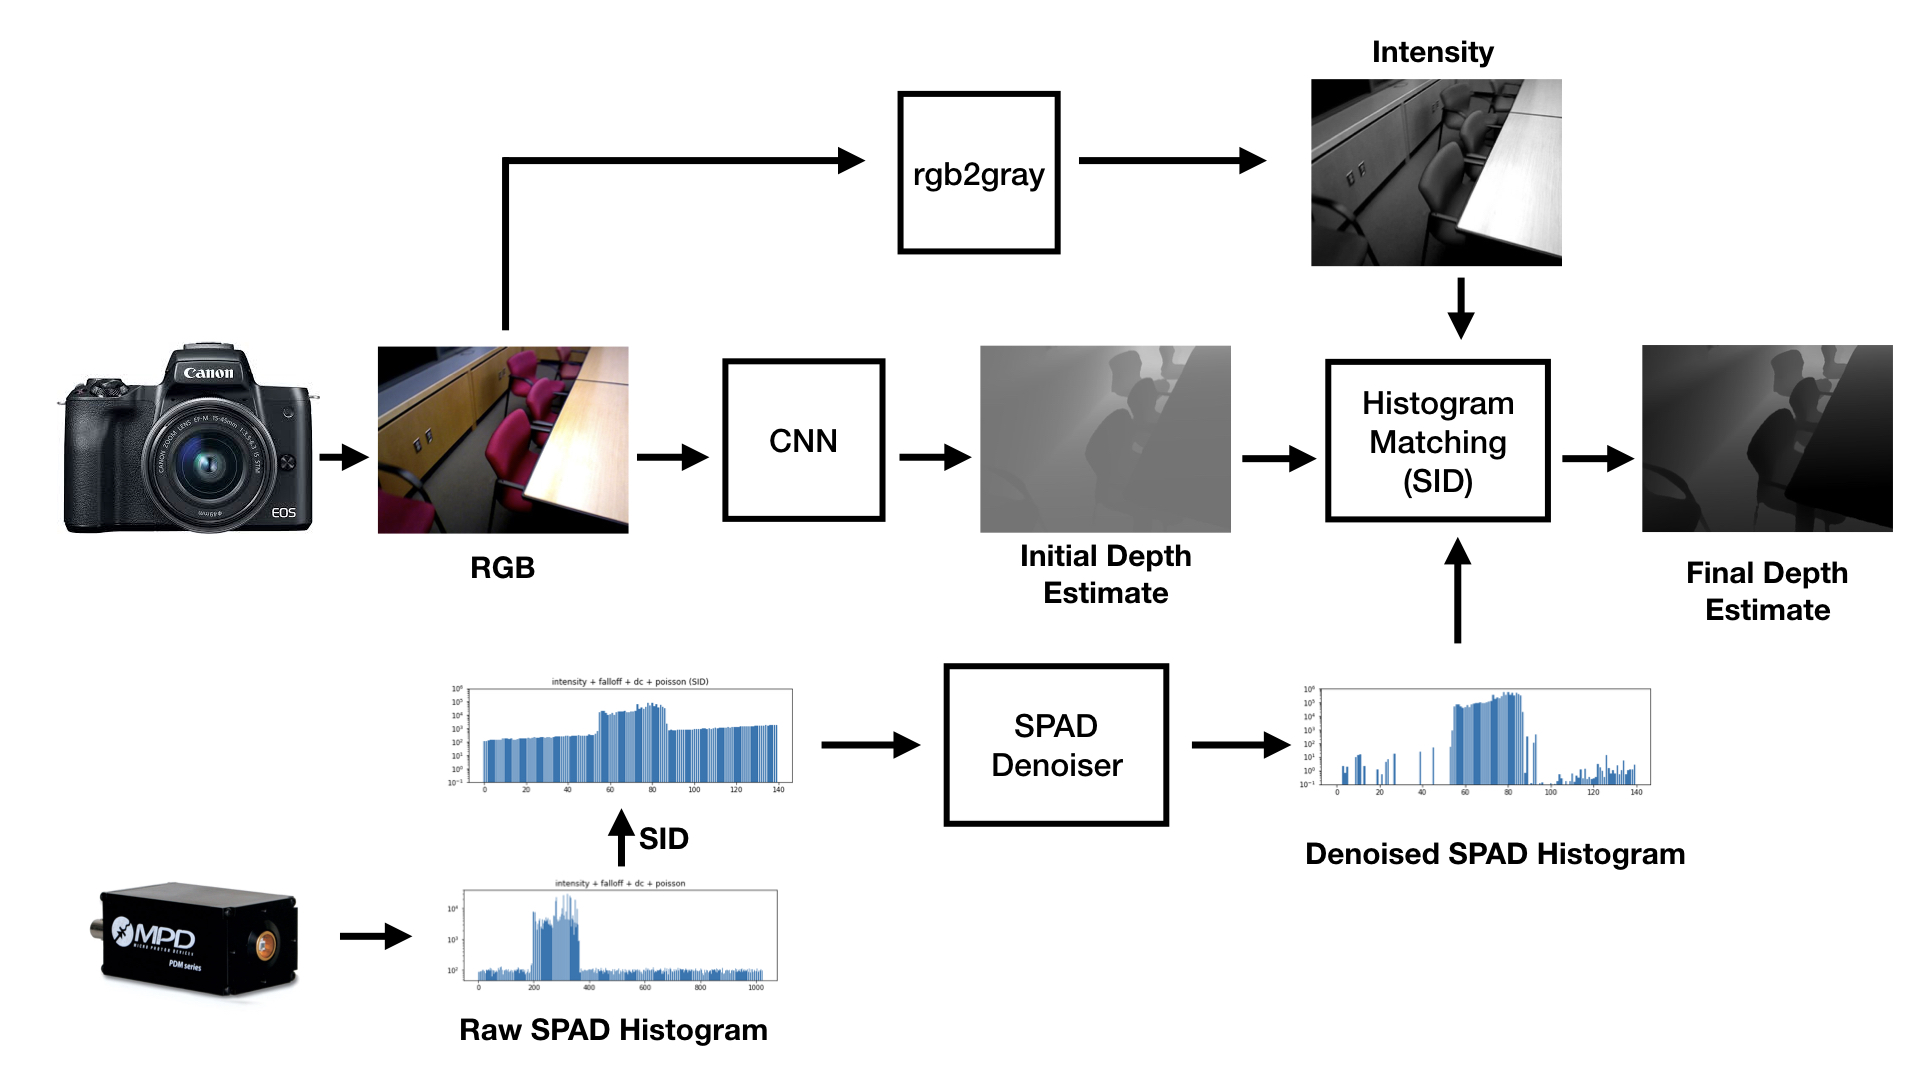
\includegraphics[height=2.5in]{full_pipeline.jpeg}
  \caption{\textbf{Overview of the full pipeline} We use a CNN to get an initial
  per-pixel depth estimate. Then we perform exact histogram matching using
  intensity-weighted pixel values on the corrected SPAD data.}
\end{figure*}
An image's \textit{histogram} is a pair of vectors $(h, b)$ where $h_i$ is the number of
pixels of the image whose value lies in the range $[b_i, b_i+1)$.
Then, given a source image $S$ with histogram $(h_s, b)$ and a target histogram
$(h_t, b)$, histogram matching generates a new image $M$ such that $h_m \approx
h_t$ and the pixel values in $M$ are in the same relative order as in $S$.
The full details of the exact histogram matching algorithm can be found in
\cite{Morovic2002}.

\begin{algorithm}[H]
 \caption{Exact Histogram Matching} 
 \label{alg:ehm}
 \begin{algorithmic}[1]
  \Procedure{ExactHistogramMatching}{$I$, $W$, $t$}
  \State $s \gets \text{Histogram}(I, W)$
  \State $M \gets \text{zeros}(rows=\text{length(s)}, cols=\text{length}(t)))$ 
  \For{$i$ in $1,...,\text{length}(s)$}
    \For{$j$ in $1,...,\text{length}(j)$}
      \State $c_t \gets \sum_{\ell = 1}^{i-1} M_{\ell j}$
      \State $c_s \gets \sum_{\ell = 1}^{j-1} M_{i \ell}$
      \State $M_{ij} \gets \min(s_i - c_s, t_j - c_t)$
    \EndFor
  \EndFor
  \State $\hat I \gets \text{zeros}(\text{shape}(I))$
  \For{each pixel $p = I_{ij}$}
    \State $d = \frac{M_{p,:}}{\text{sum}(M_{p,:})}$ \Comment{$d$ is a
      probabilty distribution}
    \State Sample $q \in \set{1,...,length(t)}$ according to $d$.
    \State $\hat I_{ij} \gets q$
  \EndFor
  \State \textbf{return} $\hat I$
  \EndProcedure
\end{algorithmic}
  
\end{algorithm}


However, for our purposes, we need to modify our algorithm to accommodate
differing per-pixel weights. We can account for squared depth falloff

\subsection{Implementation Details}
For the Monocular Depth Estimator, we use pretrained versions of the
the Deep Ordinal Regression Network (DORN) \cite{} and the DenseDepth Network.
The exact histogram matching method is as described in \cite{}.


